

%\newcommand{\gr}{\greektext}
%\newcommand{\en}{\latintext}
%\newtheorem{theorem}{Θεώρημα}[subsection]
%\newtheorem{definition}[theorem]{Orism'os}
%\newenvironment{proof}[1][áðïäåéîç]{\textsc{#1.} }{\ \rule{0.5em}{0.5em}}


%%_________________________________
\section{Εισαγωγή}

\subsection{Κρυπτοσυστήματα}

Ας υποθέσουμε ότι δύο άτομα απομακρυσμένα μεταξύ τους θέλουν να επικοινωνήσουν με τέτοιο τρόπο που κανείς άλλος να μην μάθει τι είπανε. Επειδή είναι απομακρυσμένοι, το μήνυμα αναγκαστικά θα ταξιδέψει κι έτσι θα είναι εκτεθειμένο σε οποιονδήποτε. Μια λύση για να το προστατέψουν είναι να το διαμορφώσουν έτσι ώστε ακόμα και αν κάποιος το δει, να μην μπορεί να καταλάβει τι λέει. Αυτό το σκοπό εξυπηρετούν τα διάφορα κρυπτοσυστήματα.

Ένα κρυπτοσύστημα είναι μια συνάρτηση $f_{E}:\cal P \rightarrow C$ από το σύνολο των απλών μηνυμάτων $\cal P$ στο σύνολο $\cal C$ των κρυπτογραφημάτων. Αυτή συνήθως εξαρτάται από κάποιες παραμέτρους τις οποίες ονομάζουμε <κλειδί> του κρυπτοσυστήματος. Η συνάρτηση $f_{E}$ είναι δημοσίως γνωστή, ενώ το κλειδί Ε κρατείται μυστικό. Επίσης η αντίστροφη $f^{-1}_{E}\equiv f_{D}$ καλείται συνάρτηση αποκρυπτογράφησης, με αντίστοιχο κλειδί $D$ και είναι επίσης δημοσίως γνωστή.
 
Ένα παράδειγμα είναι το κρυπτοσύστημα του Καίσαρα σύμφωνα με το οποίο κρυπτογραφούμε κάθε μήνυμα χωριστά ως εξής: το $A$ γίνεται $D$, το $B$ γίνεται $E$, το  $C$ γίνεται $F$ κ.ο.κ. Αν αντιστοιχίσουμε στο Α το 1, στο Β το 2 κλπ., τότε η συνάρτηση κρυπτογράφησης είναι η $f(x)=x+3 \ mod\ 26$ και η συνάρτηση αποκρυπτογράφησης είναι η $f^{-1}(x)=x-3\ mod\ 26$. Γενικότερα θα μπορούσαμε να έχουμε το κρυπτοσύστημα $f_{b}(x)=x+b\ mod\ 26, f^{-1}_{b}(x)=x+(-b)\ mod\ 26$, με κλειδί κρυπτογράφησης και αποκρυπτογράφησης το $b$.

Σε αυτό το κρυπτοσύστημα, όπως συνέβαινε και σε όλα μέχρι τη δεκαετία του '70, όπως το DES και το AES, το κλειδί για την αποκρυπτογράφηση ήταν το ίδιο με της κρυπτογράφησης, ή μπορούσε κάποιος να υπολογίσει εύκολα το ένα από το άλλο. Τέτοια κρυπτοσυστήματα ονομάζονται συμμετρικά. Για να επιτευχθεί η επικοινωνία, πρέπει οι δύο πλευρές με κάποιον τρόπο να συμφωνήσουν σε ένα κοινό κλειδί. Από την άλλη πλευρά, αν κάποιος τρίτος καταφέρει να αποκτήσει το κλειδί κρυπτογράφησης, μπορεί εύκολα να υπολογίσει και το κλειδί αποκρυπτογράφησης (και το αντίστροφο). 

\subsection{Κρυπτογραφία δημοσίου κλειδιού}

Η ιδέα πίσω από την κρυπτογραφία δημοσίου κλειδιού, την οποία πρώτοι εμπνεύστηκαν οι Diffie και Hellman το 1976, ήταν το να μην είναι εύκολο να υπολογίσει κανείς το κλειδί αποκρυπτογράφησης $D$ γνωρίζοντας το κλειδί κρυπτογράφησης $E$  (δηλαδή να μην υπάρχει αλγόριθμος πολυωνυμικού χρόνου που να το υπολογίζει). Ή αλλιώς, να είναι υπολογιστικά δύσκολο να αντιστρέψει κανείς την $f_{E}(x)$, εκτός αν κατέχει κάποια πρόσθετη πληροφορία, όπως το $D$. 

Οπότε το $E$ μπορεί να είναι δημοσίως γνωστό και μόνο το $D$ να κρατείται κρυφό. Έτσι δεν χρειάζεται να προηγηθεί συμφωνία σε κάποιο κοινό κλειδί: Κάθε πλευρά $(i)$ επιλέγει το ιδιωτικό (κρυφό) κλειδί $d_{i}$, και υπολογίζει και δημοσιοποιεί το αντίστοιχο δημόσιο $e_{i}$. Φυσικά αυτός ο υπολογισμός θα πρέπει να είναι εφικτός, αλλά όπως είπαμε ήδη, η εύρεση του $d_{i}$ από το $e_{i}$ πρέπει να είναι υπολογιστικά δύσκολη.

Για να στείλει ο Bob (B) ένα μήνυμα στην Alice (A), κρυπτογραφεί με το $e_{A}$. Σύμφωνα με τα παραπάνω, κανείς δεν θα μπορεί να διαβάσει το μήνυμα του Β, εκτός από την Α, η οποία είναι η μόνη που γνωρίζει το κλειδί αποκρυπτογράφησης $d_{A}$. Φυσικά ο Β δεν χρειάζεται να γνωρίζει το $d_{A}$. Τώρα αν η Α θέλει να απαντήσει στον Β, θα κρυπτογραφήσει με το $e_{B}$ και μόνο ο Β θα μπορεί να διαβάσει το μήνυμα, χρησιμοποιώντας το $d_{B}$.


\paragraph{Παρατήρηση 1}Στην πράξη τα κρυπτοσυστήματα δημοσίου κλειδιού χρησιμοποιούν κλειδιά πολύ μεγαλύτερου μήκους από αυτά της συμμετρικής κρυπτογραφίας. Επιπλέον η κρυπτογράφηση στην πρώτη περίπτωση είναι πιο χρονοβόρα διαδικασία από ότι στην δεύτερη, ειδικά όταν έχουμε μηνύματα μεγάλου μήκους.

Για αυτόν το λόγο η κρυπτογραφία δημοσίου κλειδιού συνήθως χρησιμοποιείται για να επιτευχθεί η συμφωνία σε ένα κοινό κλειδί, το οποίο στη συνέχεια θα χρησιμοποιηθεί σε ένα σύστημα συμμετρικής κρυπτογραφίας.

Για παράδειγμα ένα πρωτόκολλο ανταλλαγής κλειδιού που βασίζεται σε κρυπτογραφία δημοσίου κλειδιού είναι το πρωτόκολλο Diffie Hellman, που βασίζεται στη δυσκολία του διακριτού λογαρίθμου, δηλ. της αντιστροφής της $f(x)=g^x \mod p$ όπου $p$ πρώτος:

 Έστω $ Z_p $ και $ g \in Z_p $ ένα δημόσια γνωστό στοιχείο. Αν η Αλίκη και ο Βασίλης θέλουν να συμφωνήσουν ένα κοινό κρυφό κλειδί, μπορούν να κάνουν τα εξής:
\begin{enumerate}
\item Η Αλίκη διαλέγει τυχαία και μυστικά ένα στοιχείο $ \alpha \in \{2,\dots,p-1\} $, υπολογίζει το $ g^\alpha \mod p $ και το στέλνει στον Βασίλη.
\item Ο Βασίλης διαλέγει τυχαία και μυστικά ένα στοιχείο $ \beta \in \{2,\dots,p-1\} $, υπολογίζει το $ g^\beta \mod p $ και το στέλνει στην Αλίκη.
\item Η Αλίκη υπολογίζει το $ k_\alpha = \left( g^\beta\right)^\alpha \mod p$.
\item Ο Βασίλης υπολογίζει το $ k_\beta = \left( g^\alpha\right)^\beta \mod p$.
\item Το κοινό κλειδί είναι το $ k = k_\alpha = k_\beta $.
\end{enumerate}


\paragraph{Παρατήρηση 2}Όπως αναφέραμε, τα κρυπτοσυστήματα δημοσίου κλειδιού βασίζουν την ασφάλειά τους στη δυσκολία αντιστροφής μιας συνάρτησης $f$, εκτός αν υπάρχει γνώ-ση μιας επιπλέον πληροφορίας. Τέτοιες συναρτήσεις λέγονται συναρτήσεις καταπακτής (trapdoor functions). Παρεμφερής είναι και η έννοια της συνάρτησης μονής κατεύθυνσης (one way function). Έτσι ονομάζεται μια συνάρτηση, με την ιδιότητα ότι είναι εύκολο να βρεις την τιμή της σε ένα σημείο, αλλά είναι δύσκολο να την αντιστρέψεις.

Είναι ανοιχτό πρόβλημα αν υπάρχουν τέτοιες συναρτήσεις. Αυτό συνδέεται με προβλήματα της θεωρίας πολυπλοκότητας, τα οποία είναι ακόμα ανοιχτά μετά από δεκαετίες προσπαθειών να απαντηθούν. Ένα τέτοιο πρόβλημα είναι η εικασία $P\neq NP$. Τελικά αυτά τα κρυπτοσυστήματα βασίζουν την ασφάλειά τους στο γεγονός ότι \emph{μέχρι τώρα} δεν έχει βρεθεί πολυωνυμικού χρόνου αλγόριθμος που να αντιστρέφει τις συναρτήσεις που χρησιμοποιούν.   

Τα τελευταία χρόνια έχουν προταθεί πολλά κρυπτοσυστήματα που βασίζονται σε προβλήματα της θεωρίας ομάδων. 

%%\subsection{Βασικά Στοιχεία Κρυπτογραφίας}
%%
%%Στα βασικά κρυπτογραφικά σχήματα δύο άτομα, η Αλίκη και ο Βασίλης, θέλουν να επικοινωνήσουν ασφαλώς μέσω ενός μη ασφαλούς %%καναλιού (μίας ασύρματης σύνδεσης ή μέσω τηλεφώνου). Αν η Αλίκη και ο Βασίλης κατέχουν μία πληροφορία που μόνο αυτοί
%%ξέρουν (ένα κοινό μυστηκό κλειδί) μπορούν να το χρησιμοποιήσουν, μαζί με ένα συμμετρικό κρυπτοσύστημα όπως το AES %%%%%%%%(Advanced Encryption Standard) για να επικοινωνήσουν. Αν δεν έχουν, μπορούν να εκτελέσουν ένα προτόκολο ανταλλαγής %%κλειδιού, όπως το Diffie-Hellman για να αποκλείσουν ένα μυστικό κλειδί ή να χρησιμοποιήσουν ένα κρυπτοσύστημα δημοσίου %%%%κλειδιού, όπως το RSA ή το ElGamal που δεν απαιτεί την ύπαρξη μυστικού κλειδιού. 

% one way funcions
%dh
%dlp

%%
%%Πριν προχωρήσουμε υπάρχουν δύο στοιχεια που πρέπει να τονιστούν για κάθε κρυπτοσύστημα:
%%\begin{itemize}
%%\item\textbf{H Αλίκη και ο Βασίλης είναι μηχανές}
%%	Άρα ο στόχος είναι η παραγωγή ενός προτοκόλου που είναι καλά προσδιορισμένο ώστε να μπορεί να υλοποιηθεί. %%%%%%%%%%%%Συγκεκριμένα, ένα καλά προσδιορισμένο σχήμα πρέπει να περιγράφει ....
%%\item\textbf{H ασφάλεια είναι πολύ λεπτή έννοια}
%%\end{itemize}

\section{Κρυπτογραφία με χρήση Ομάδων}

Θα περιγράψουμε κάποια σχήματα που έχουν προταθεί, τα οποία χρησιμοποιούν μη αβελιανές ομάδες (μη αντιμεταθετικές), όπως αυτά παρουσιάζονται στο \cite{basic}. Το δύσκολο πρόβλημα στο οποίο βασίζουν την ασφάλειά τους είναι το πρόβλημα της συζυγίας.

\subsection{Συζυγία και Ύψωση σε Δύναμη}
Έστω $ G $ μια μη αβελιανή ομάδα. Για $ g,x \in G $ ορίζουμε 
\begin{align*}
g^x &= x^{-1}gx
\end{align*}
τον συζυγή του $ g $ με τον $ x $. Αυτή η γραφή υπονοεί ότι η συζυγία μπορεί να χρησιμοποιηθεί αντί της ύψωσης σε δύναμη στην κρυπτογραφία. Έτσι, μπορούμε να ορίσουμε το ανάλογο πρόβλημα του διακριτού λογαρίθμου:
\paragraph*{Πρόβλημα Αναζήτησης συζηγους:} Έστω $ G $ μία μη αβελιανή ομάδα. Έστω $ g,h \in G $ τέτοια ώστε $ h=g^x $ για κάποιο άγνωστο $ x\in G $. Δοσμένων των $ g $ και $ h$, βρες ένα στοιχείο $ y \in G $ τέτοιο ώστε $ h = g^y $. Ή με τον άλλο συμβολισμό, δεδομένων των $g,h$ βρες $y$ τ.ω. $h=y^{-1}gy$.

Αν βρούμε κάποια ομάδα στην οποία το Πρόβλημα Αναζήτησης Συζυγούς είναι υπολογιστικά δύσκολο (και τα στοιχεία της ομάδας είναι εύκολο να τα αποθηκεύσουμε και να τα διαχειριστούμε) τότε μπορούμε να ορίσουμε κρυπτοσυστήματα ανάλογα αυτών που στηρίζονται στο πρόβλημα του διακριτού λογαρίθμου. Οι Ko et al. πρότειναν το ακόλουθο ανάλογο του πρωτοκόλλου ανταλλαγής κλειδιού Diffie-Hellman.
\label{ko}
\paragraph*{Πρωτόκολλο ανταλλαγής κλειδιού Ko-Lee-Cheon-Han-Kang-Park \cite{ko}} Έστω $ G $ μια μη αβελιανή ομάδα και $ g \in G $ ένα δημόσια γνωστό στοιχείο της $ G $. Έστω $ A,B $ δύο commuting υποομάδες της $ G $,
%δηλ. $ [a,b]=1 $, 
δηλ. τα $a,b$ αντιμετατίθενται για κάθε $ a \in A, b \in B $. Αν η Αλίκη και ο Βασίλης θέλουν να συμφωνήσουν ένα κοινό κρυφό κλειδί, μπορούν να κάνουν τα εξής:
\begin{enumerate}
\item Η Αλίκη διαλέγει τυχαία και μυστικά ένα στοιχείο $ \alpha \in A $, υπολογίζει το $ g^\alpha = \alpha^{-1} g \alpha $ και το στέλνει στον Βασίλη.
\item Ο Βασίλης διαλέγει τυχαία και μυστικά ένα στοιχείο $ \beta \in B $, υπολογίζει το $ g^\beta = \beta^{-1} g \beta $ και το στέλνει στην Αλίκη.
\item Η Αλίκη υπολογίζει το $ k_\alpha = \left( g^\beta\right)^\alpha $.
\item Ο Βασίλης υπολογίζει το $ k_\beta = \left( g^\alpha\right)^\beta $.
\item Το κοινό κλειδί είναι το $ k = k_\alpha = k_\beta $, αφού $\alpha\beta=\beta\alpha$.
\end{enumerate}

Πρέπει να παρατηρήσουμε ότι τα $k_{\alpha},k_{\beta}$ μπορεί να έχουν διαφορετική αναπαράσταση, και γενικά δεν είναι εύκολο να ελέγξει κανείς αν δύο στοιχεία με διαφορετική αναπαράσταση ταυτίζονται. Οπότε χρειαζόμαστε ομάδες των οποίων τα στοιχεία να μπορούν να γραφτούν σε μία (μοναδική) κανονική μορφή. Η ομάδες που έχουν προταθεί για αυτό το πρωτόκολλο είναι οι ομάδες πλεξίδων (braid groups), τις οποίες θα παρουσιάσουμε αργότερα.

Μία παραλλαγή του πρωτοκόλλου  είναι το ακόλουθο των Anshel, Anshel και Goldfeld που έχει το πλεονέκτημα ότι οι commuting υποομάδες $ A $ και $ B $ δεν χρειάζονται.

\paragraph*{Πρωτόκολλο ανταλλαγής κλειδιού Anshel-Anshel-Goldfeld \cite{Anshel99analgebraic}} Έστω $ G $ μια μη αβελιανή ομάδα και έστω τα στοιχεία $ \alpha_1, \dots, \alpha_k,\beta_1, \dots, \beta_m \in G $ δημόσια γνωστά στοιχεία της $ G $. Αν η Αλίκη και ο Βασίλης θέλουν να συμφωνήσουν ένα κοινό κρυφό κλειδί, μπορούν να κάνουν τα εξής:
\begin{enumerate}
\item Η Αλίκη διαλέγει τυχαία και μυστικά ένα στοιχείο $ x \in \alpha_1, \dots, \alpha_k $, υπολογίζει τα $ \beta_1^x, \dots, \beta_m^x $ και τα στέλνει στον Βασίλη.
\item Ο Βασίλης διαλέγει τυχαία και μυστικά ένα στοιχείο $ y \in \beta_1, \dots, \beta_m $, υπολογίζει τα $ \alpha_1^y, \dots, \alpha_k^y $ και τα στέλνει στην Αλίκη.
\item Η Αλίκη υπολογίζει το $ k_\alpha = x^y $.
\item Ο Βασίλης υπολογίζει το $k_\beta= y^x$.
\item Το κοινό κλειδί είναι το $ k =[x,y] = x^{-1}y^{-1} xy  
= x^{-1}k_\alpha = \left( y^{-1} k_\beta \right)^{-1} $ \label{key}
\end{enumerate}

Από το βήμα 5 φάινεται ότι δεν είναι απαραίτητο να λύσει η Alice (ή ο Bob αντίστοιχα) το πρόβλημα της συζυγίας, για να μπορέσει να βρει το $y$ (το $x$ ο Bob αντίστοιχα) και να υπολογίσει το κλειδί.

Για αυτό το πρωτόκολλο προτάθηκε και πάλι η χρήση των Braid groups, λόγω (α) της ύπαρξης κανονικής μορφής, και (β) της δυσκολίας του προβλήματος της συζυγίας σε αυτές τις ομάδες. Παρακάτω θα δώσουμε συνοπτικά και άλλες πιθανές ομάδες που έχουν προταθεί να χρησιμοποιηθούν σε αυτά τα πρωτόκολλα.


\subsection{Platform groups}

Για να είναι ασφαλές κάποιο ``κανονικό'' κρυπτογραφικό πρωτόκολλο (που στηρίζεται σε one-way συνάρτηση), πρέπει η group platform πάνω στην οποία υλοποιείται να ικανοποιεί κάποιες απαιτήσεις. Για το \ref{ko} οι απαιτήσεις αυτές μπορούν να διατυπωθούν ως εξής:
\begin{enumerate}
\item Η ομάδα πρέπει να είναι γνωστή ή/και να έχει μελετηθεί αρκετά.
\item Ο υπολογισμός του κλειδιού πρέπει να είναι υπολογιστικά εύκολος.
\item Το πρόβλημα αναζήτησης συζυγούς πρέπει να είναι υπολογιστικά δύσκολο.
\item Το πλήθος των λέξεων μήκους $ n $ της ομάδας, πρέπει να είναι υπερεκθετικό του $ n $. 
\end{enumerate}
Η ύπαρξη των τριών πρώτων απαιτήσεων είναι προφανής. Η τέταρτη απαίτηση εισάγεται για να αποκλειστεί το ενδεχόμενο το πρόβλημα Αναζήτησης συζυγούς να λυθεί αποδοτικά με την εξαντλητική (brute-force) μέθοδο.

Στην συνέχεια της ενότητας θα παρουσιάσουμε έξι ομάδες που ικανοποιούν τις απαιτήσεις αυτές, άρα μπορούν να χρησιμοποιηθούν για την υλοποίηση των πρωτοκόλλων \ref{ko}. Θα δώσουμε έμφαση στις Braid groups, ενώ τις υπόλοιπες θα αναφέρουμε επιγραμματικά.

\subsubsection{Braid Groups}

Η braid group στο $ n $ συμβολίζεται με $ B_n $, είναι μία άπειρη ομάδα για $ n>1 $. Τα braid groups έχουν μελετηθεί εκτενώς \cite{normaf,normaltheor,nfobs} και έχουν την ακόλουθη γεωμετρική ερμηνεία.
Θεωρούμε δύο ραβδιά με  $ n $ καρφιά η καθεμία, το ένα απέναντι από το άλλο, έτσι ώστε κάθε καρφί του ενός ραβδιού να βρίσκεται απέναντι από κάποιο καρφί του άλλου. Χρησιμοποιώντας νήματα, συνδέουμε κάθε καρφί του ενός ραβδιού με κάποιο του άλλου  δημιουργώντας μία ένα-προς-ένα αντιστοιχία. Συχνά κάποιο νήμα θα πρέπει να περάσει κάτω ή πάνω από κάποιο άλλο, μία ή περισσότερες φορές, και αυτό είναι σημαντικό, αφού οι ακόλουθες πλεξίδες είναι διαφορετικές:

%%\fbox{
%%$$
%%\xy 0;/r1pc/:+(0,-2)
%%,(0,0)*={\xoverh};
%%(0,-3);(1,-3) **@{-};
%%(0,-2);(1,-2) **@{-}
%%\endxy
%%$$ 
%%}
%%\fbox{
%%$$
%%\xy 0;/r1pc/:+(0,-2)
%%,(0,0)*={\xunderh};
%%(0,-3);(1,-3) **@{-};
%%(0,-2);(1,-2) **@{-}
%%\endxy
%%$$ 
%%}

\begin{figure}[ht]
\center{
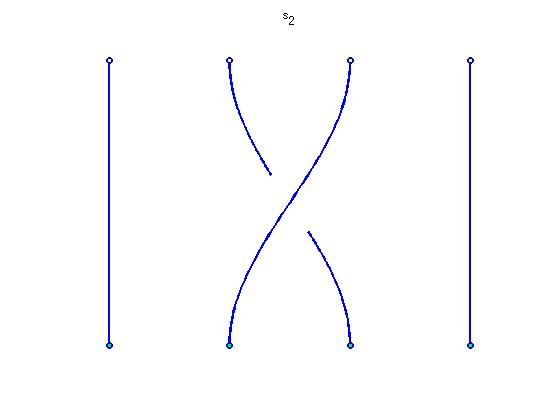
\includegraphics[width=60mm]{2.jpg}
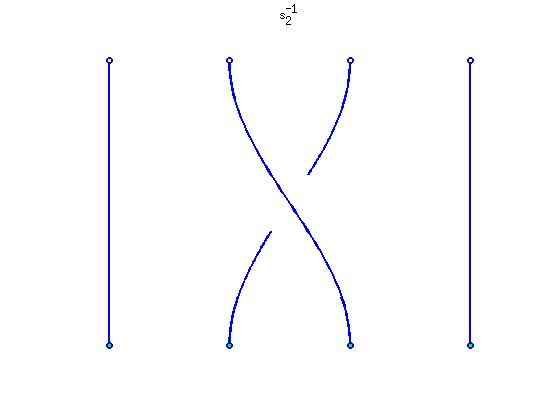
\includegraphics[width=60mm]{_2.jpg}
}
\caption{Braids $\sigma_2$ και $\sigma_2^{-1} $}
\label{bdio}
\end{figure}

Οι γεννήτορες της ομάδας  συμβολίζονται με $\sigma_{j},  0<j<n$, και $\sigma_{j}$ είναι η πλεξίδα που ενώνει κάθε καρφί με το απέναντί του, εκτός από το $j$-οστό που το ενώνει με το $j+1$, ενώ το $j+1$ με το $j$, και επιπλέον το $j$-οστό νήμα τοποθετείται κάτω από το $j+1$. Αντίστροφό του είναι το $\sigma_{j}^{-1}$, όπου τα δύο νήματα διασταυρώνονται αντίθετα, όπως στο Σχήμα \ref{bdio}, που βλέπουμε τα $\sigma_{2},\sigma_{-2}, (n=4)$.    


 Αν ενώσουμε δύο braids $ u $ και $ v $ στην σειρά τότε παίρνουμε ένα καινούργιο, το $ uv $, άρα η συνένωση συμβολίζει τον πολλαπλασιασμό. Για παράδειγμα, στο Σχήμα \ref{benaenatria} βλέπουμε την $\sigma_{1}\sigma_{1}\sigma_{3}$.

\begin{figure}[h]
\center{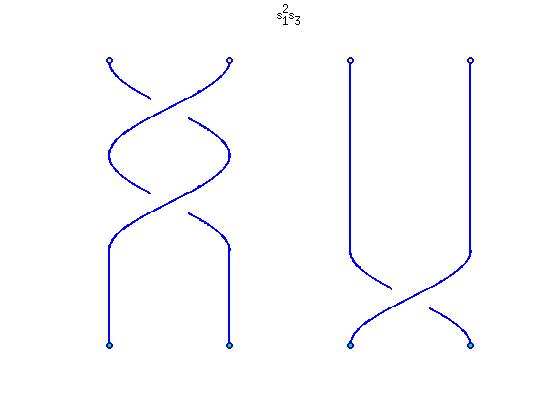
\includegraphics[width=60mm]{113.jpg}} 
\caption{Braid $ \sigma_{1}\sigma_{1}\sigma_3 $}
\label{benaenatria}
\end{figure}

Σαν ουδέτερο στοιχείο της πράξης θεωρούμε αυτό που δεν περιέχει καθόλου τομές και το ονομάζουμε απλό braid, όπως στο Σχήμα \ref{bempty}.

\begin{figure}[ht]
\center{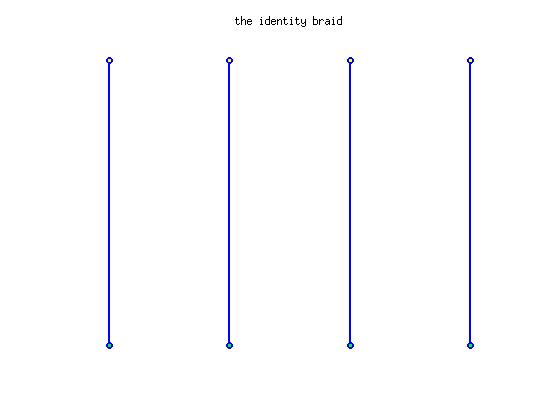
\includegraphics[width=60mm]{empty.jpg}}
\caption{Απλό braid}
\label{bempty}
\end{figure}

 Θεωρούμε δύο braids ισοδύναμα αν είναι δυνατό να δημιουργήσουμε από το ένα το άλλο μετακινώντας τα νήματα στον χώρο χωρίς να αλλάζουμε τα άκρα τους. Το σύνολο $ B_n $ είναι το σύνολο των κλάσεων ισοδυναμίας των braids με $ n $ νήματα και έχει δομή ομάδας αφού αν πολλαπλασιάσουμε κάποιο braid με την αντανάκλασή (τον αντίστροφό) του το αποτέλεσμα είναι ισοδύναμο με το απλό braid. 

Ουσιαστικά κάθε braid είναι μία ακολουθία τομών. Ονομάζουμε μια τομή θετική αν το μπροστινό νήμα έχει θετική κλίση (όπως η $\sigma_{2}$), διαφορετικά την ονομάζουμε αρνητική (όπως η $\sigma_{-2}$). 

Εύκολα προκύπτει ότι ισχύουν τα εξής:

\begin{align*}
[\sigma_i,\sigma_j]=1, 
\end{align*}
για κάθε $ i,j $ τέτοια ώστε $ \mid i-j \mid>1 $
και
\begin{align*}
x_i x_{i+1} x_i=x_{i+1}x_ix_{i+1} 
\end{align*}
για κάθε $ i $ τέτοιο ώστε $ 1 \leq i \leq n-2 $

Στην πραγματικότητα οι δύο αυτές σχέσεις αρκούν για να περιγράψουν την $ B_n $.

Permutation braid έχουμε όταν όλες οι τομές της πλεξίδας είναι θετικές, και κάθε δύο νήματα διασταυρώνονται το πολύ μία φορά, όπως στο Σχήμα \ref{bedet} που φαίνεται η $\sigma_{1}\sigma_{2}\sigma_{1}\sigma_{3}$ που αντιστοιχεί στην permutation 4213. H permutation braid που αντιστοιχεί στην μετάθεση 4321 (γενικά στην μετάθεση n,n-1,...,2,1), λέγεται fundamental braid και θα την συμβολίζουμε με $\Delta$ και φαίνεται στο Σχήμα \ref{delta}.
\begin{figure}[h]
\center{
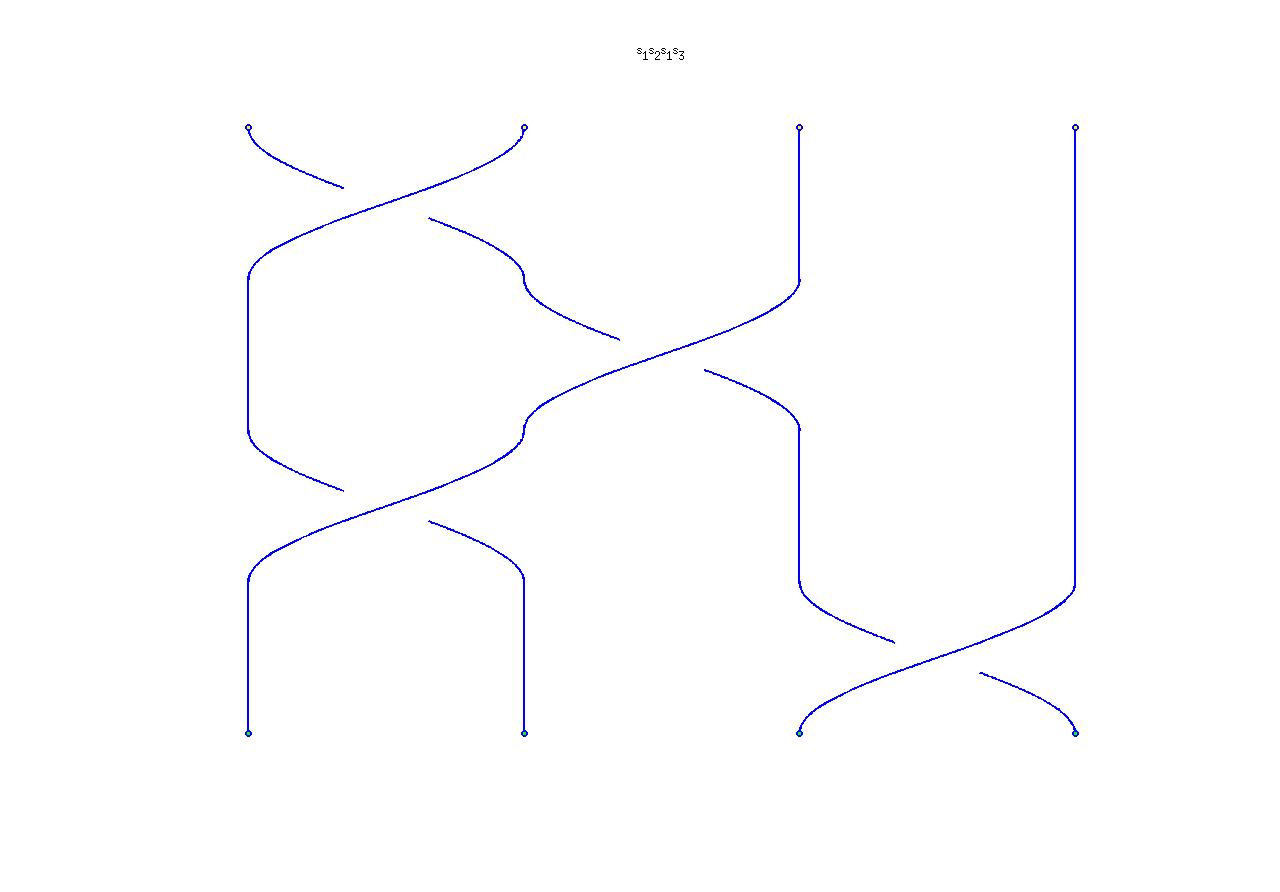
\includegraphics[width=60mm]{1213.jpg}
}
\caption{Braid $ \sigma_1\sigma_2\sigma_1\sigma_3 $}
\label{bedet}
\end{figure}

\begin{figure}[h]
\center{
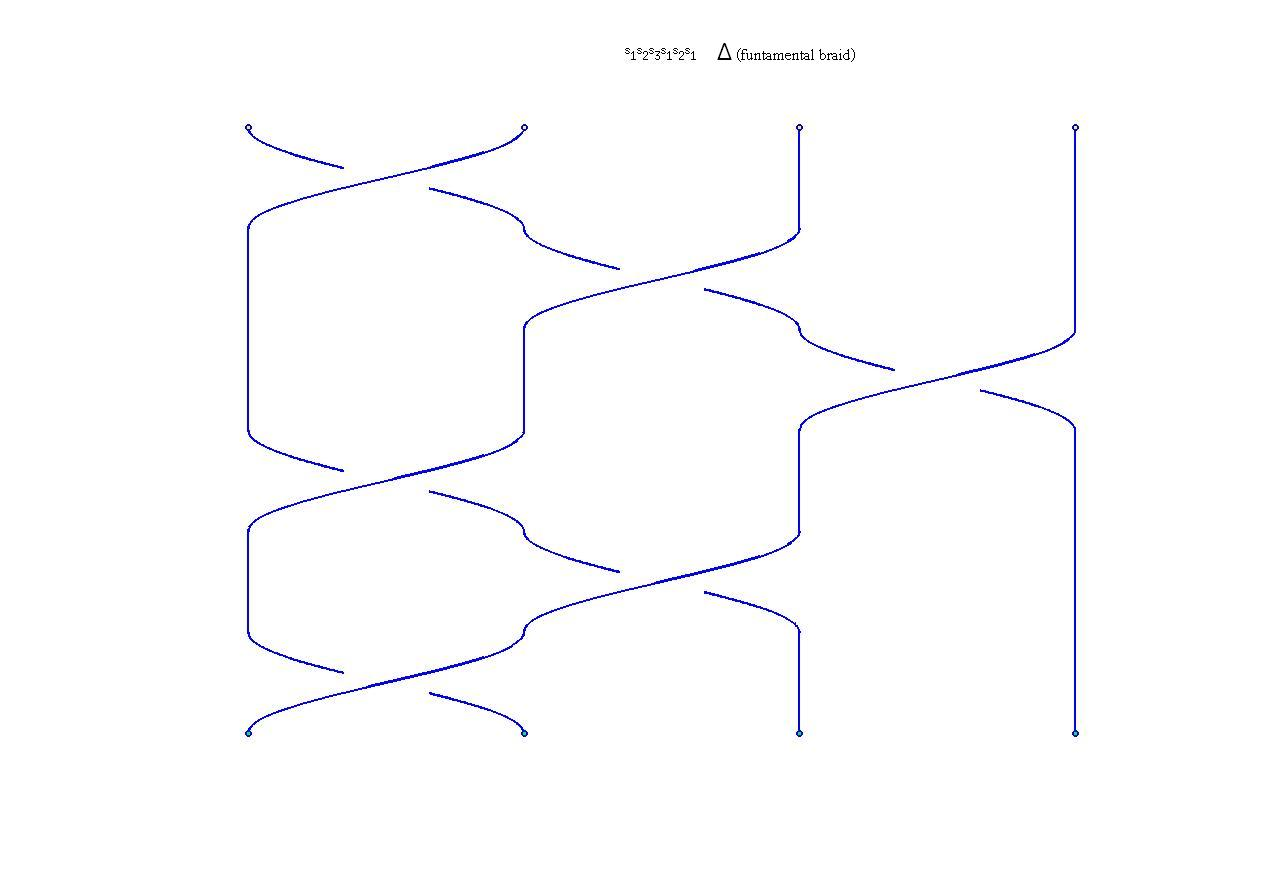
\includegraphics[width=60mm]{delta.jpg}
}
\caption{Briad $ \Delta $}
\label{delta}
\end{figure}
Το σύνολο των permutation braids, θα το συμβολίζουμε με $\Sigma_{n}$. 

 Για την $ B_n $ υπάρχουν αρκετές γνωστές κανονικές μορφές, οι πιο γνωστές εκ των οποίων είναι οι Dehornoy handle free form και η Garside normal form. 
Για την Dehornoy handle free form  δεν υπάρχει καλή θεωρητική εκτίμηση πολυπλοκότητας, όμως στην πράξη δουλεύει σε γραμμικό χρόνο, ενώ η Garside normal form τρέχει σε τετραγωνικό χρόνο.
H  ύπαρξη πολλών κανονικών μορφών μπορεί να προκαλέσει πρόβλημα, αφού κάποια κανονική μορφή μπορεί να ;αποκαλύπτει πληροφορίες που κάποια άλλη προσπαθεί να αποκρύψει. Συγκεκριμένα, έχει αποδειχτεί ότι η μετατροπή από την Garside στην Dehornoy κανονική μορφή κάνει τις υποκείμενες μεταδόσεις πιο επιρρεπείς σε επιθέσεις.

Η δυσκολία του προβλήματος της συζυγίας φαίνεται να ικανοποιείται, αν και παρά τις μελέτες που έχουν γίνει είναι ακόμα άγνωστο αν το πρόβλημα αναζήτησης συζηγούς ανήκει στο NP.
Τελικά, όσον αφορά την ιδιότητα 4 το πλήθος των $ B_n, n\geq 2 $ έχουν εκθετική αύξηση. Για $ n\geq 3 $ αυτό προκύπτει από το γεγονός ότι η $ B_n $ έχει ελεύθερες υποομάδες, για παράδειγμα οι $ \sigma_1^2 $ και $ \sigma_2^2 $ παράγουν μια ελεύθερη υποομάδα.

\paragraph{Παρατηρήσεις}
\begin{enumerate}
\item Έστω $B_n^+$ το σύνολο των θετικών πλεξίδων (δηλ. των πλεξίδων που όλες οι τομές είναι θετικές). Για μία θετική πλεξίδα $P$ ορίζουμε το starting set, και το finishing set
\[S(P)=\{i|P=\sigma_i P'\ for\ some\ P'\in B_n^+ \}\]
\[F(P)=\{i|P=P'\sigma_i \ for\ some\ P'\in B_n^+ \}.\]
Για μία permutation braid A που αντιστοιχεί στην permutation $\pi$ (όπου $\pi(i)=j$ αν το $i$ καρφί του πάνω ραβδιού ενώνεται με το $j$ του κάτω) ισχύει 
\[S(A)=\{i|\pi(i)>\pi(i+1)\}\]
\[F(A)=\{i|\pi^{-1}(i)>\pi^{-1}(i+1)\}.\]
Για παράδειγμα, για την Δ στην φωτογραφία $S(\Delta)=F(\Delta)=\{1,2,3\}$, ενώ για την $A=\sigma_{1}\sigma_{2}\sigma_{1}\sigma_{3}$ είναι $S(A)=\{1,2\},F(A)=\{1,3\}$.

\item Για την Δ πλεξίδα ισχύουν τα εξής
	\begin{enumerate}[(i)]
	\item $\forall 0<j<n, \Delta=\sigma_j A_j=B_j \sigma_j$ για κάποιες permutation braids $A_j,B_j$.
	\item $\forall 0<i<n, \sigma_i\Delta=\Delta\sigma_i$.
	\end{enumerate}
Άρα σε κάθε λέξη (πλεξίδα) $W$ από $\sigma_i$, μπορούμε να αντικαταστήσουμε τα $\sigma_i^{-1}$ με τον τύπο $\sigma_i^{-1}=\Delta^{-1}B_i$ από την πρώτη ιδιότητα, και χρησιμοποιώντας την δεύτερη ιδιότητα, να φέρουμε τα Δ στην αρχή. Έτσι παίρνουμε την έκφραση $W=\Delta^u P, P\in B_n^+$. 

\item Για κάθε θετική λέξη $P$ υπάρχει μία μοναδική αποσύνθεση που λέγεται left-weighted decomposition, ως εξής
\[P=A_1 P_1, A_1\in\Sigma_n, P_1\in B_n^+, S(P_1)\subset F(A_1). \]
Επαναλαμβάνοντας την ίδια διαδικασία για το $P_1$ κ.ο.κ. και φέρνοντας τα Δ στην αρχή, παίρνουμε την αριστερή κανονική μορφή Garside, η οποία είναι μοναδική για κάθε πλεξίδα
\[P=\Delta^u A_1 A_2 ...A_p, u\in Z, A_{i}\in\Sigma_n\setminus\{e,\Delta\}.\] 
\end{enumerate}

Από τις παραπάνω παρατηρήσεις προκύπτει το εξής θεώρημα κανονικής μορφής.

\begin{thm} 
Για κάθε $W\in B_n$ υπάρχει μία μοναδική αναπαράσταση, που λέγεται αριστερή κανονική μορφή 
\[P=\Delta^u A_1 A_2 ...A_p, u\in Z, A_{i}\in\Sigma_n\setminus\{e,\Delta\},\] 
όπου $A_i A_{i+1}$ είναι left-weighted για κάθε $0<i<n$. Το $p$ ορίζεται ως το μήκος Garside $l(W)$. 
\end{thm}


\paragraph{Παρατήρηση}
Αποδεικνύεται ότι η παραπάνω κανονική μορφή μπορεί να υπολογιστεί σε χρόνο $O(l^2 n\log n)$, όπου $l$ το μήκος της λέξης σε μη κανονική μορφή. Επίσης αποδεικνύεται ότι το πλήθος των n-braids κανονικού μήκους p είναι τουλάχιστον $(\lfloor\frac{n-1}{2}\rfloor !)^p$. 

%see ref 
% a group G is called free if there is a subset S of G such that any element of G can be written in one and only one way as a product of finitely many elements of S and their inverses (disregarding trivial variations such as st−1 = su−1ut−1). Apart from the existence of inverses no other relation exists between the generators of a free group.

\subsubsection{Thompson's group}

Η ομάδα F του Thomson \cite{belk-2007} είναι μία άπειρη μη αβελιανή ομάδα που είναι γνωστή σε πολλούς κλάδους των μαθηματικών, όπως η άλγεβρα, η γεωμετρία και η ανάλυση. Για τον λόγω αυτό, η ομάδα έχει μελετηθεί εκτενώς και μπορεί να προταθεί για την υλοποίηση των \ref{ko}.

Η ομάδα αυτή μπορεί να περιγραφεί με χρήση γεννητόρων και σχέσεων ορισμού ως 

\begin{align*}
F&=\left\langle x_0, x_1, x_2  \mid x_i^{-1}x_kx_i = x_{k+1} \ (k>i) \right\rangle
\end{align*}
Όπως και στις braid ομάδες, στην ομάδα F υπάρχουν πολλές κανονικές μορφές, όμως η ``κλασική'' κανονική μορφή ενός στοιχείου $ w $ μπορεί να υπολογιστεί σε χρόνο $ O(\mid w \mid \log{\mid w \mid}) $, άρα ικανοποιείται και η 2 ιδιότητα.

Όσον αφορά την 3η ιδιότητα αν και στο \cite{cf} αποδεικνύεται ότι υπάρχει αποδοτική λύση για την επίλυση του ταυτόχρονου προβλήματος του συζυγούς στο F, το πρόβλημα ιδιότητας μέλους παραμένει απρόσιτο, συνεπώς δεν υπάρχει αλγόριθμος που να επιτρέπει σε κάποιον αντίπαλο αποδοτικά να υπολογίσει το κλειδί.

Όσον αφορά την 4η ιδιότητα μπορεί να δειχθεί \cite{tom} ότι ικανοποιείται.

\subsubsection{Ομάδες Πινάκων}

Σαν πλατφόρμα για την υλοποίηση των \ref{ko} μπορούν να χρησιμοποιηθούν ομάδες πινάκων πάνω σε πεπερασμένους αντιμεταθετικούς δακτύλιους αφού αυτές έχουν ότι συνδυάζουν τα πλεονεκτήματα και τα μειονεκτήματα της αντιμεταθετικότητα. Συγκεκριμένα, ο πολλαπλασιασμός πινάκων είναι μη αντιμεταθετικός, αλλά τα στοιχεία των πινάκων προέρχονται από αντιμεταθετικό δακτύλιο και συνεπώς μπορούν να παρέχουν μία ``φυσική'' κανονική μορφή.

Ο συνδυασμός αντιμεταθετικότητας των στοιχείων των πινάκων και μη-αντιμεταθετι-κότητας του πολλαπλασιασμού είναι πολύ σημαντικό συστατικό της ασφάλειας του συστήματος, αφού απαγορεύει στον εισβολέα να χρησιμοποιήσει προφανείς σχέσεις όπως η $ ab=ba $ για να απλοποιήσει γινόμενα.

\subsubsection{Άλλες Ομάδες}

Άλλες ομάδες που μπορούν να χρησιμοποιηθούν είναι οι small cancellation groups, solvable groups, Artin groups, Grogorchuck's group.



\section{Κρυπτανάλυση}
Σε αυτήν την ενότητα θα αναφέρουμε κάποιες επιθέσεις στο πρόβλημα της συζυγίας στις Braid groups. Το 1969 ο Garside \cite{attack} έδωσε έναν αλγόριθμο για την εύρεση αν δύο στοιχεία της ομάδας είναι συζυγή, κατασκευάζοντας για κάθε στοιχείο $x$ ένα υποσύνολο $I_x$ (που ονομάζεται summit set) τ.ω. τα $x,y $ είναι συζυγή αν και μόνο αν $I_x=I_y$. Το πρόβλημα είναι ότι τα summit sets μπορεί να ήταν εκθετικά μεγάλα.

Άλλη επίθεση (των Hofheinz και Steinwandt \cite{Hattack}) βασίζεται στην παρατήρηση ότι οι αντιπρόσωποι δύο συζυγών μέσα σε μία ειδική κατηγορία υποσυνόλων που λέγονται super-summit sets, είναι συζυγείς μέσω μίας permutation braid.

\subsection{Επιθέσεις βασισμένες στο μήκος}
\label{analysis}
Στην περίπτωση των πρωτοκόλλων που παρουσιάσαμε, δεν ψάχνουμε να βρούμε αν δύο λέξεις είναι συζυγείς, αλλά αυτό το γνωρίζουμε. Το πρόβλημα του επιτιθέμενου είναι δοθέντων δύο πλεξίδων $x, z=y^{-1}xy$, να βρει το $y$. Ο αλγόριθμος που χρησιμοποιούμε παρουσιάζεται στο \cite{length-basedattacks}.

Θεωρούμε μία συνάρτηση μήκους $l(x)$, όπως το μήκος της κανονικής μορφής. Αν υποθέσουμε ότι $y=y'\sigma_i$ με $l(y')<l(y)$, τότε για κάθε $j\neq i, l(\sigma_i z \sigma_i^{-1})<l(\sigma_j z \sigma_j^{-1})$, γιατί $\sigma_i z \sigma_i^{-1}=  \sigma_i y^{-1}xy  \sigma_i^{-1}= \sigma_i  \sigma_i^{-1} y'^{-1}xy'\sigma_i\sigma_i^{-1}=y'^{-1}xy'$.

Οπότε βρίσκουμε το $\sigma_i$ και επαναλαμβάνουμε το ίδιο για το $z'=y'^{-1}xy'$ κ.ο.κ. Για να βρούμε το $\sigma_i$ βρίσκουμε όλα τα $l(\sigma_j z \sigma_j^{-1})$ και παίρνουμε το μικρότερο. Αν είναι πολλά ίσα, τότε τα ελέγχουμε όλα. 

Όσον αφορά στο χρόνο εκτέλεσής του αλγορίθμου, επειδή σε κάθε βήμα βρίσκει κάποιο $\sigma_i$ της αναπαράστασης του $y$, τερματίζει σε χρόνο γραμμικό στο μήκος της μη κανονικής μορφής του $y$, σε αντίθεση με την εξαντλητική μέθοδο, που θα χρειαζόταν χρόνο εκθετικό στην κανονική μορφή του $y$, όπως προκύπτει από την παρατήρηση για την κανονική μορφή. 

Ο αλγόριθμος δεν επιτυγχάνει πάντα και αυτό οφείλεται σε δύο λόγους. 

Ο πρώτος είναι ότι επιλέγεται πάντα κάποιο $ j $ τέτοιο ώστε το μήκος του $l(\sigma_j z \sigma_j^{-1})$ να ελαχιστοποιηθεί. Το ότι το $ j $ αυτό θα είναι σωστό δεν είναι εξασφαλισμένο. Για να αντιμετωπιστεί το πρόβλημα αυτό θα έπρεπε να ελέγχονταν όλα τα $ j $ που ικανοποιούν την $l(y')<l(y)$, με $y=y'\sigma_i$, όμως τότε ο χρόνος εκτέλεσης του αλγορίθμου θα ήταν κοντά στον χρόνο εκτέλεσης του brute force αλγορίθμου. 

Ο δεύτερος λόγος είναι ότι ο αλγόριθμος μπορεί να επιτύχει, δηλαδή να επιστρέψει κάποιο $ y' $ τέτοιο ώστε $ y'^{-1}xy'=z $, όμως να μην ισχύει $ y=y' $, όπως φαίνεται στο ακόλουθο παράδειγμα.
Για $ y= \sigma_1^{-4}$ και $ g=\sigma_3^2\sigma_1\sigma_3 $ ο αλγόριθμος επιστρέφει $ y'=\sigma_3^4 $ και ισχύει $ y'^{-1}xy'=y^{-1}xy=\Delta^{-8}[ 2     1     4     3][ 1     2     4     3][ 1     2     4     3] $, δηλαδή τα δύο αυτά στοιχεία έχουν την ίδια κανονική μορφή.
Έτσι όταν χρησιμοποιήσουμε αυτήν την επίθεση για να βρούμε το κλειδί $a^{-1}b^{-1}gba=b^{-1}a^{-1}gab$, εάν έχουμε βρει ένα $a'$ τ.ω. $a'^{-1}ga'=a^{-1}ga$, τότε υπάρχουν δύο περιπτώσεις: 

Αν το $a'$ περιέχει στοιχεία μόνο από το υποσύνολο του $ B_n $ από το οποίο επιτρέπεται να κατασκευαστεί το $ a $ τότε δεν υπάρχει πρόβλημα, αφού το σύνολο αυτό αντιμετατίθεται με το με στοιχεία του συνόλου από τα οποία επιτρέπεται να κατασκευαστεί το κλειδί $ b $, άρα βρίσκουμε το σωστό κλειδί. Διαφορετικά, μπορεί να μην αντιμετατίθεται με το $b$, κι έτσι προκύπτει διαφορετικό κλειδί.

Εύκολα προκύπτει ότι η πιθανότητα επιτυχίας είναι τουλάχιστον $ 1/O(n^l) $, όπου $ l$ το μήκος του $ a $, και αφού το μήκος αυτό είναι σταθερό, η πιθανότητα είναι $ 1/poly(n) $.

Τέλος, το ποσοστό επιτυχίας του εξαρτάται σημαντικά από την συνάρτηση μήκους που χρησιμοποιείται.


%Η επιτυχία του αλγορίθμου δεν είναι εξασφαλισμένη και ο βαθμός επιτυχίας του εξαρτάται σημαντικά από την συνάρτηση μήκους.  


\section{Υλοποίηση}
Σε αυτήν την εργασία σχεδιάσαμε και υλοποιήσαμε αλγόριθμο εύρεσης κανονικής μορφής των πλεξίδων της ομάδας $B_4$
 ($n=4$). Στη συνέχεια υλοποιήσαμε τα πρωτόκολλα της ενότητας 2, πάνω σε αυτήν την ομάδα. Επίσης προσπαθήσαμε να υλοποιήσουμε επιθέσεις στο πρόβλημα της συζυγίας. Η μία επίθεση που επιχειρήσαμε είναι η εξαντλητική, ενώ η άλλη είναι αυτή που αναφέραμε στην προηγούμενη ενότητα (δηλ. την βασισμένη στο μήκος), χρησιμοποιώντας σαν συνάρτηση μήκους το Garside μήκος της λέξης. 

%%%%%%%%%%%%%%%%%%%%%%%%%%%%%%%%%%%%%%%%%%%%%%%%%%%%%%%%%%%%%%%%%%%%%